\section{IDS and anomaly detection}
\label{chap:IDS}
An intrusion can be defined as an unauthorised activitiy that causes damage to an information system: essentially, any attack that could pose a possible threat to the information confidentiality, integrity or availability is an intrusion.

An IDS (Intrusion Detection System) is a software or hardware system that identifies malicious actions on information systems in order to allow for system security to be maintained.
The goal of an IDS is to identify malicious network traffic and computer usage, which cannot be identified by a traditional firewall, in order that high protection against actions that compromise the availability, integrity, or confidentiality of computer systems is achieved.
IDS systems can be categorised into two groups: SIDS (Signature-based Intrusion Detection System) and AIDS (Anomaly-based Intrusion Detection System).

SIDS and AIDS systems will be described, according to Khraisat et al.'s work on IDS systems \parencite{Khraisat}, in the following subsection.

\subsection{Signature-based intrusion detection systems}
SIDS systems are based on pattern matching techniques to find a known attack: when an intrusion signature matches with the signature of a previous intrusion that already exists in the signature database, an alarm signal is triggered (host’s logs are inspected to find sequences of commands or actions which have previously been identified as malware).
The main idea consists of building a database of intrusion signatures (signatures are created as state machines, formal language string patterns or semantic conditions) and comparing the current set of activities against the existing signatures and raising an alarm if a match is found.

SIDS systems usually give an excellent detection accuracy for previously known intrusions \parencite{Kreibich} while, on the other hand, they have difficulty in detecting zero-day attacks since no matching signatures exist in the database until the signatures of the new attacks are extracted and stored.
The traditional technique used in SIDS systems consists of examining network packets and trying matching against a signature database.
Unfortunately, this technique is unable to identify attacks that span several packets: due to the advanced sophistication of modern malwares, it may be necessary to extract signature information over multiple packets (this requires the IDS systems to recall the contents of earlier packets).

The increasing rate of zero-day attacks\parencite{Symantec} has rendered SIDS techniques progressively less effective because no prior signature exists for any such attacks.
Moreover, this traditional paradigm can be further undermined by polymorphic variants of malwares and the rising amount of targeted attacks.
A potential solution to this problem would be to use AIDS techniques, which operate by profiling what is an acceptable behavior rather than what is anomalous, as described in the next subsection.

\subsection{Anomaly-based intrusion detection system}
AIDS is a system capable to overcome the limitation of SIDS: given the assumption that malicious behavior differs from typical user behavior, any significant deviation between the observed behavior and the model is regarded as an anomaly, which can be interpreted as an intrusion (so, the behaviors of abnormal users which are dissimilar to standard behaviors are classified as intrusions).

The development of an AIDS consists of two phases:
\begin{itemize}
    \item the training phase: the normal traffic profile is used to learn a model of normal behavior;
    \item the testing phase: a new data set is used to establish the system’s capacity to generalise to previously unseen intrusions.
\end{itemize}


In recent years, several AIDS approaches have been proposed for improving detection accuracy and reducing false alarms.
Thus, AIDS systems can be classified into different categories based on the method used for training (i.e., for creating a normal model of the behavior of a computer system):
\begin{itemize}
    \item statistical-based: the collection and examinination of every data record in a set of items and the building of a statistical model of normal user behavior are involved;
    \item knowledge-based: it tries to identify the requested actions from existing system data such as protocol specifications and network traffic instances;
    \item machine learning-based: complex pattern-matching capabilities are acquired from training data.
\end{itemize}

\begin{figure}[H]
\centering
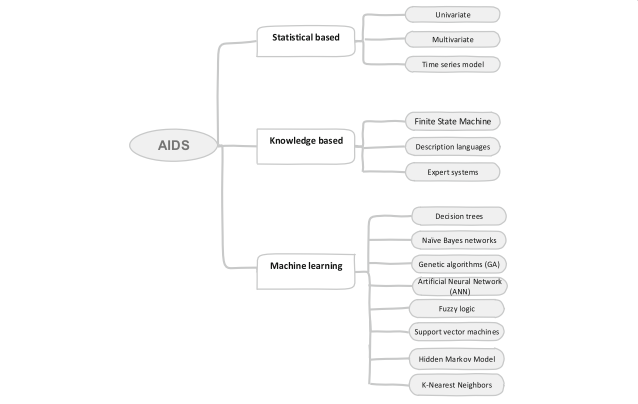
\includegraphics{Resources/AIDS.png}
\caption{Classification of AIDS methods}
\label{fig:AIDS}
\end{figure}

The main advantage of AIDS is the ability to identify zero-day attacks due to the fact that recognising the abnormal user activity does not rely on a signature database: AIDS triggers a danger signal when the examined behavior differs from the usual behavior.

Furthermore, AIDS systems have various benefits:
\begin{enumerate}
    \item they have the capability to discover internal malicious activities (e.g., if an intruder starts making transactions in a stolen account that are unidentified in the typical user activity, it creates an alarm);
    \item it is very difficult for a cybercriminal to recognise what is a normal user behavior without producing an alert as the system is constructed from customised profiles.
\end{enumerate}

To sum up, SIDS systems can only identify well-known intrusions whereas AIDS systems can detect zero-day attacks.

However, AIDS systems can result in a high false positive rate because anomalies may just be new normal activities rather than genuine intrusions.

\subsection{Statistics-based techniques}
A statistics-based IDS builds a distribution model for normal behaviour profile, then detects low probability events and flags them as potential intrusions.

Statistical AIDS systems essentially take into account the statistical metrics such as the median, mean, mode and standard deviation of packets: in other words, rather than inspecting data traffic, each packet is monitored.

Moreover, statistical AIDS are employed to identify any type of differences in the current behavior from normal behavior and are tipically based on one of the following models:
\begin{itemize}
    \item univariate (i.e., the data has only one variable): this technique is used when a statistical normal profile is created for only one measure of behaviours in computer systems; univariate IDS look for abnormalities in each individual metric.
    \item multivariate (i.e., the data has more than one variable): it is based on relationships among two or more measures in order to understand the relationships between variables; this model would be valuable if experimental data show that better classification can be achieved from combinations of correlated measures rather than analysing them separately; however, the main challenge for multivariate statistical IDs is that it is difficult to estimate distributions for high-dimensional data;
    \item time series model: a time series is a series of observations made over a certain time interval; a new observation is abnormal if its probability of occurring at that time is too low (the feasibility of this technique was validated through simulated experiments).
\end{itemize}